\documentclass{article}
\usepackage{include/nips15submit_e,times}
\usepackage{hyperref}
\usepackage{url}
\usepackage[noend]{algpseudocode}
\renewcommand\algorithmicthen{}
\renewcommand\algorithmicdo{}
\usepackage{algorithm}
\usepackage{natbib}
\usepackage{graphicx}

\definecolor{mydarkblue}{rgb}{0,0.08,0.45}
\hypersetup{
    colorlinks=true,
    linkcolor=mydarkblue,
    citecolor=mydarkblue,
    filecolor=mydarkblue,
    urlcolor=mydarkblue}

\newcommand{\vw}{\mathbf{w}}
\newcommand{\vv}{\mathbf{v}}
\newcommand{\vf}{\mathbf{f}}
\newcommand{\vg}{\mathbf{g}}
\newcommand{\vi}{\mathbf{i}}
\newcommand{\vr}{\mathbf{r}}
\newcommand{\vzero}{\mathbf{0}}
\newcommand{\ones}[1]{\mat{1}_{#1}}
\newcommand{\eye}[1]{\mat{E}_{#1}}
\newcommand{\tra}{^{\mathsf{T}}}
\newcommand{\vect}[1]{{\bf{#1}}}
\newcommand{\mat}[1]{\mathbf{#1}}
\newcommand{\pderiv}[2]{\frac{\partial #1}{\partial #2}}
\newcommand{\npderiv}[2]{\nicefrac{\partial #1}{\partial #2}}

\title{Neural Molecular Fingerprints}

\author{
David Duvenaud\\
Harvard University\\
\texttt{dduvenaud@seas.harvard.edu}
\And
Dougal Maclaurin\\
Harvard University\\
\texttt{maclaurin@physics.harvard.edu}
\And
Ryan P. Adams\\
Harvard University\\
\texttt{rpa@seas.harvard.edu}
}

%\nipsfinalcopy % Uncomment for camera-ready version
\begin{document}
\maketitle

\begin{abstract}
Predicting properties of molecules requires functions that take graphs as inputs.
Molecular graphs are usually processed using off-the-shelf hash-based functions which compute fixed-size fingerprint vectors, which are then fed into standard machine learning methods.
We introduce a generalization of commonly-used molecular fingerprints based on convolutional neural networks which allow learning of the entire feature pipeline.
\end{abstract}

\section{Introduction}

Much progress has recently been made by the application of deep learning to virtual screening, where the task is to predict the properties of novel molecules by generalizing from examples.
One difficulty with this task is that the input to the predictor, a molecule, can be of arbitrary size and shape.
Most machine learning pipelines can only handle inputs of a fixed size.
The formula followed by \cite{unterthinerdeep}, \cite{unterthiner2015toxicity}, and \cite{ramsundar2015massively} was to use off-the-shelf fingerprint software to compute fixed-dimensional feature vectors, using those as inputs to standard fully-connected deep neural networks.
The networks are optimized using gradient descent, but the molecular fingerprints and treated as fixed.

In this paper, we replace the fixed molecular fingerprints with fully differentiable neural networks, whose inputs are graphs representing the original molecule.
In these graphs, vertices represent individual atoms, and edges represent bonds.
Th

Neural fingerprints offer several advantages over fixed fingerprints:
\begin{itemize}
\item Better predictive performace ???
\item Because fixed fingerprints are not adapted to the task at hand, their output vector must be extremely large to encode all possible substructures without overlap.
For example, \cite{unterthinerdeep} used a fingerprint vector of size 43,000 for each molecule, after having removed rarely-occurring features in order to make the problem computationally feasible.
We [hopefully] show that better performance can be achieved using feature vectors a fraction of the size, reducing memory requirements and computational burden.
\item Finally, the architecture presented here opens the door for more sophisticated information-aggregation architectures, such as recursive neural networks [cite].
\end{itemize}

\subsection{Desirable Properties of Molecular Representations}

\begin{itemize}
\item invariant to global orientation
\item invariant to atom re-labeling
\item invariant to the SMILES representation (at the very least)
\item NOT invariant to reordering locally (maintain information about the orientation)
    example:  fragment1 - C - O - fragment2 is not the same as fragment1 - O - C - fragment2 
   \item speed
\end{itemize}

\cite{erhan2006collaborative}
\cite{ma_qsar_2015}

\section{Dealing with local ordering}

Morgan fingerprints deal with local ordering by having a canonical order.



\section{Extended-connectivity fingerprints}

\begin{figure}
\centerline{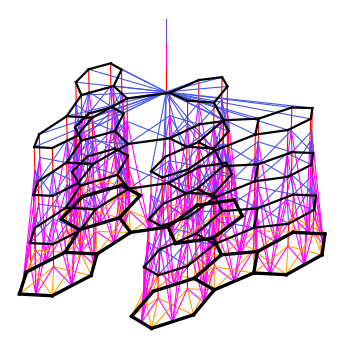
\includegraphics[width=0.4\textwidth]{figures/3d-nets/net1}}
\caption{A visualization of one of the convolutional nets constructed on a molecule.}
\label{placeholder}
\end{figure}

\begin{figure}
\centerline{
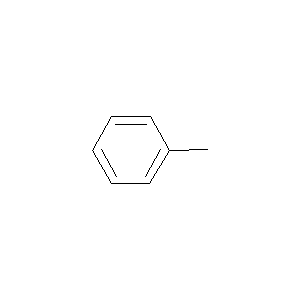
\includegraphics[width=0.2\textwidth]{figures/convnet-features/hidden-unit-0}
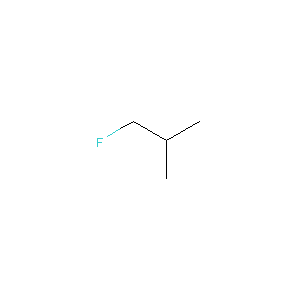
\includegraphics[width=0.2\textwidth]{figures/convnet-features/hidden-unit-1}}
\caption{The molecular fragments which most activate two of the features of the convolutional net.}
\label{placeholder}
\end{figure}




\begin{figure*}[t]
 \begin{minipage}[t]{0.49\columnwidth}
 \begin{algorithm}[H]
\caption{Circular fingerprints} 
\label{alg:ecfp} 
\begin{algorithmic}[1]
\State \textbf{Input:} {molecule, radius $R$, size $S$}
\State \textbf{Initialize:} {fingerprint vector $\vf \leftarrow \vzero_S$}
\For {each atom $a$ in molecule} 
    \State $\vr_a \leftarrow g(a)$ \Comment {lookup atom features}
\EndFor
\For {$L = 1$ to $R$} \Comment {for each layer}
	\For {each atom $a$ in molecule}
		\State $\vr_{n1} \dots \vr_{nN} = \textnormal{neighbors}(a)$
		\State $\vv \leftarrow [\vr_a \vr_{n1} \dots, \vr_{nN}]$ \Comment {concatenate}
		\State $\vr_a \leftarrow \textnormal{hash}(\vv)$ \Comment {hash function}
		\State $i \leftarrow \textnormal{mod}(r_a, S)$ \Comment {convert to index}		
		\State $\vf_{i} \leftarrow 1$ \Comment {Write 1 at index}
	\EndFor
\EndFor
\State \textbf{Return:} {binary vector $\vf$}
\end{algorithmic}
\end{algorithm}
\end{minipage}
\hfill
\begin{minipage}[t]{0.49\columnwidth}
\begin{algorithm}[H]
\caption{Neural fingerprints} 
\label{alg:neural} 
\begin{algorithmic}[1]
\State \textbf{Input:} {molecule, radius $R$, size $S$, {\color{blue} $\theta_1 \dots \theta_R$}}
\State \textbf{Initialize:} {fingerprint vector $\vf \leftarrow \vzero_S$}
\For {each atom $a$ in molecule} 
	\State $\vr_a \leftarrow g(a)$ \Comment {lookup atom features}
\EndFor
\For {$L = 1$ to $R$} \Comment {for each layer}
    \For {each atom $a$ in molecule}
		\State $\vr_{n1} \dots \vr_{nN} = \textnormal{neighbors}(a)$
		\State $\vv \leftarrow [\vr_a \vr_{n1}, \dots \vr_{nN}]$ \Comment {concatenate}
		\State $\vr_a \leftarrow {\color{blue} \vf_{\theta_L}}(v)$ \Comment {{\color{blue} smooth function}}
		\State $\vi \leftarrow \textnormal{{\color{blue}softmax}}(\vr_a)$ \Comment {{\color{blue} sparsify}}
		\State $\vf \leftarrow {\color{blue} \vf + \vi}$ \Comment {{\color{blue}add to fingerprint}}
    \EndFor
\EndFor
\State \textbf{Return:} { {\color{blue} real-valued} vector $\vf$}
\end{algorithmic}
\end{algorithm}
\end{minipage}
\hfill
\caption{Pseudocode of circular fingerprints (\emph{left}) and neural fingerprints (\emph{right}).
Differences are highlighted in blue.
Every non-differentiable operation has been replaced with a differentiable analogue.}
\end{figure*}




\section{Related work}

\paragraph{Fingerprints}

[Cite Morgan] and \cite{ECFP2010} developed extended circular fingerprints.
These fingerprints map identical molecules to the same set of fingerprints.
These same fingerprints have been pressed into service as a measure of similarity.

However, for a meaningful measure of similarity, 

\paragraph{Convolutional Neural Networks}

Convolutional neural networks have been used to model images, speech, and time series\cite{lecun1995convolutional}.
However, standard convolutional architectures use a fixed computational graph, making them difficult to apply to objects of varying size or structure, such as molecules.
More recently, \cite{KalchbrennerACL2014} developed a convolutional neural network architecture for modeling sentences of varying length and structure.

\paragraph{Recursive Neural Networks}

\cite{socher2011semi} and \cite{socher2011dynamic} use a pyramidal architecture for performing inference on variable-length sentences.

\paragraph{Neural nets for QSAR}

\cite{ramsundar2015massively} Massively multitask networks for drug discovery

\cite{dahl2014multi} used standard deep neural networks, and didn't do any feature engineering.

\paragraph{Machine learning for identifying promising molecules}

\cite{Eckert2007225, bergeron2011modeling} provide reviews of the field.
\cite{tingley2014towards} used a variety of standard machine learning algorithms to predict the photovoltaic efficiency of organic molecules.

\paragraph{Neural Networks on Graphs}

\cite{graphnn2009} The Graph Neural Network Model

\cite{micheli2009neural} Neural network for graphs



\section{Experiments}

[How much is conceptual purity worth?  We can try using only topology, or include lots of hand-engineered features that we think will be useful.]

\subsection{Are Morgan fingerprints basically a hash function for molecules?}

We can answer this question by evaluating the performance of neural fingerprints generated by randomly initialized weights.


\subsection{Datasets}

Tripod dataset: \url{https://tripod.nih.gov/tox21/challenge/}
\cite{unterthiner2015toxicity}


\subsection{Software}

\subsection{Implementation Details}
Automatic differentiation (AD) software packages such as
Theano~\citep{Bastien-Theano-2012, bergstra2010scipy} significantly speed up development time by providing gradients automatically, but can only handle limited control structures and indexing.
Since we required relatively complex control flow and indexing in order to implement variants of Algorithm \ref{alg:neural}, we implemented our own automatic differentiation package for Python, available at \url{<redacted>}.
This package differentiates standard Numpy~\citep{oliphant2007python} code, and can differentiate code containing
while loops, branches, indexing, and even its own gradient evaluations.

Code for all experiments in this paper will be made available upon publication.



\section{Extensions}

\paragraph{How much computation to perform at each layer?}
i.e. how complicated should we make the function that goes from one layer of the graph to the next?

\paragraph{Building parse trees}
For the pyramidal architecture, we need to decide on a parse tree of the molecule.
One way to do this in a 'soft' way might be to max-pool over many different local parsings.
This could be done at multiple layers, which would limit the exponential blowup.

\paragraph{Preserve asymmetries explicitly or implicitly}
If we tie the weights of all neighboring vertices, then ordering information is lost locally, although it is still preserved implicitly in the relations between nodes in the next layer.

\subsection{Interpretability}
[Idea: Use nested dropout to allow a variable-sized descriptor.]
Explain that it's analogous to PCA for neural nets

[Wishlist: Include figures showing which fragments maximally activate different features - hopefully showing that they correspond to interpretable, familiar concepts]

\section{Conclusions}


\section*{acknowledgments}
This work was partially supported by a grant from the Spanish Ministry of Science and Technology.



\subsubsection*{References}

\bibliography{references.bib}
\bibliographystyle{include/icml2015}



\end{document}